\documentclass[12pt, oneside]{article}
\usepackage[letterpaper, margin=1.0in, headsep=0.1in, headheight=43pt]{geometry}
\usepackage[english]{babel}
\usepackage[utf8]{inputenc}
\usepackage{amsmath}
\usepackage{amsfonts}
\usepackage{amssymb}
\usepackage{tikz}
\usepackage{pgfplots}
\pgfplotsset{width=10cm,compat=1.9}
%\usepgfplotslibrary{statistics}
%\usepackage{pgfplotstable}

\usepackage{tkz-fct}

\usepackage{fancyhdr}
\pagestyle{fancy}
\fancyhf{}
\rhead{Name: \hspace{.75in} }
\lhead{BECA / Dr. Huson / Algebra 2 \\* 30 May 2019 \\* Homework: Polynomial function features \& graphing}

\renewcommand{\headrulewidth}{0pt}

\title{Worksheet and test template}
\author{Chris Huson}
\date{March 2018}

\begin{document}
Use pencil for graphs. Label points as ordered pairs.
\begin{enumerate}

\item The function $f(x)=x^3-3x^2-2x+2$
      is shown on the graph.

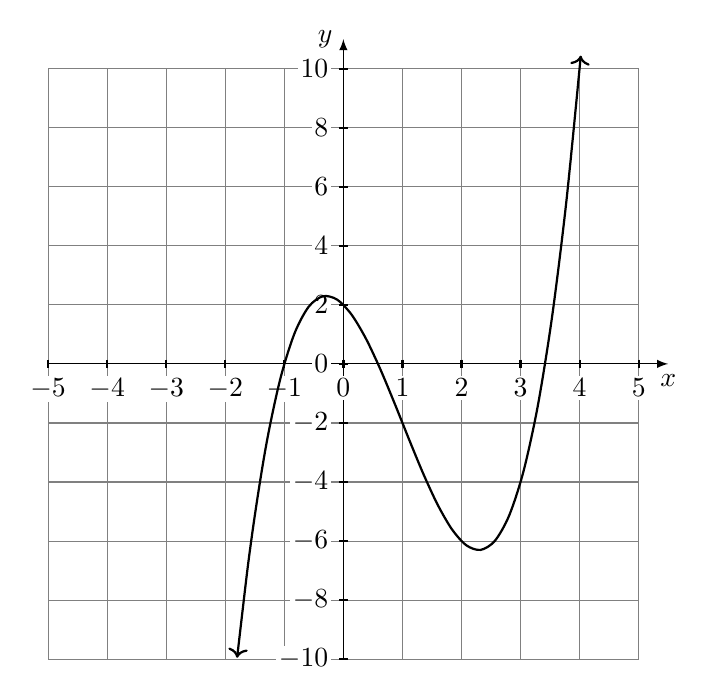
\begin{tikzpicture}[scale=.75]
  \tkzInit[xmin=-5,xmax=5,ymin=-10,ymax=10,ystep=2]
  \tkzGrid
  \tkzAxeXY
  %\tkzFct[color=blue,thick,domain = -5:5]{x**3-3*x**2-2*x+2};
  \draw [<->,thick,smooth,domain=-1.8:4.02] plot(\x,{0.5*((\x)^3-3*(\x)^2-2*(\x)+2)});
\end{tikzpicture}

\begin{enumerate}
    \item Write down the $y$-intercept.
    \item Show that $f(0)$ is the $y$-intercept by substituting $x=0$ into the function $f(x)$.\\*[20pt]
    \item Write down the $x$-intercepts.
    \item Show that $-1$ is an $x$-intercept because $x=-1$ is a solution to $f(x)=0$.\\*[20pt]
    \item What is the end behavior?
    \begin{enumerate}
        \item As $x\xrightarrow{}+\infty$ does $y\xrightarrow{}+\infty \text{ or } -\infty$?
        \item As $x\xrightarrow{}-\infty$ does $y\xrightarrow{}+\infty \text{ or } -\infty$?
    \end{enumerate}
    \item Label the local maximum and local minimum as ordered pairs (approximate the values).
    \item Slope: on the $x$-axis below, label the portion of the domain where $f$ is increasing with pluses (``+") and decreasing with negative signs (``-"). Mark the extema (maximum and minimum) with zeros since $f(x)$ is horizontal at those points.
    \item Write down the intervals the function is increasing and decreasing.\\*[10pt]
\end{enumerate}

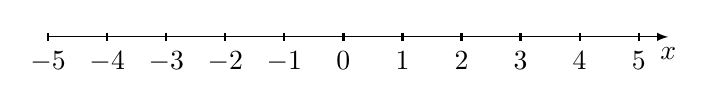
\begin{tikzpicture}[scale=.75]
  \tkzInit[xmin=-5,xmax=5]
  \tkzAxeX
\end{tikzpicture}

\newpage
\item Plot the function $g(x)=-x^3-5x^2-3x+4$ on the graph.

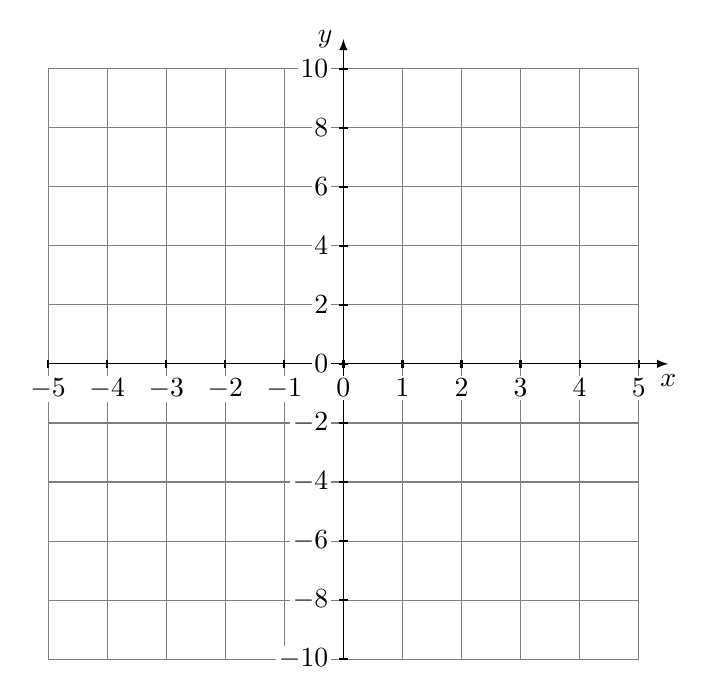
\begin{tikzpicture}[scale=.75]
  \tkzInit[xmin=-5,xmax=5,ymin=-10,ymax=10,ystep=2]
  \tkzGrid
  \tkzAxeXY
  \tkzFct[color=blue,thick,domain = -5:5]{-x**3-5*x**2-3*x+4};
\end{tikzpicture}

\begin{enumerate}
    \item Write down the $y$-intercept.
    \item Show that $f(0)$ is the $y$-intercept by substituting $x=0$ into the function $f(x)$.\\*[20pt]
    \item Write down the $x$-intercepts.
    \item Show that $-4$ is an $x$-intercept because $x=-4$ is a solution to $f(x)=0$.\\*[20pt]
    \item What is the sign of the leading coefficient?\\* What is the end behavior?
    \begin{enumerate}
        \item As $x\xrightarrow{}+\infty$ does $y\xrightarrow{}+\infty \text{ or } -\infty$?
        \item As $x\xrightarrow{}-\infty$ does $y\xrightarrow{}+\infty \text{ or } -\infty$?
    \end{enumerate}
    \item Label the local maximum and local minimum as ordered pairs (approximate the values).
    \item Slope: on the $x$-axis below, label the domain as increasing, decreasing, or horizontal (with ``+", ``-", \& ``0"), and state the respective intervals. \\*[10pt]
\end{enumerate}

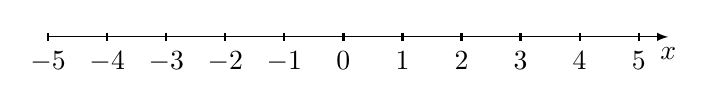
\begin{tikzpicture}[scale=.75]
  \tkzInit[xmin=-5,xmax=5]
  \tkzAxeX
\end{tikzpicture}

\newpage
\item Given the function $h(x)=-x^3-2x^2+5x+6$.

\begin{enumerate}
    \item Write down the $y$-intercept. Mark it on the plot.
    \item Show that $-1$ is an $x$-intercept because $x=-1$ is a solution to $f(x)=0$. Mark $(-1, 0)$ on the graph as an $x$-intercept.\\*[20pt]
    \item The other $x$-intercepts are $-3$ and $+2$. Mark them on the plot.

    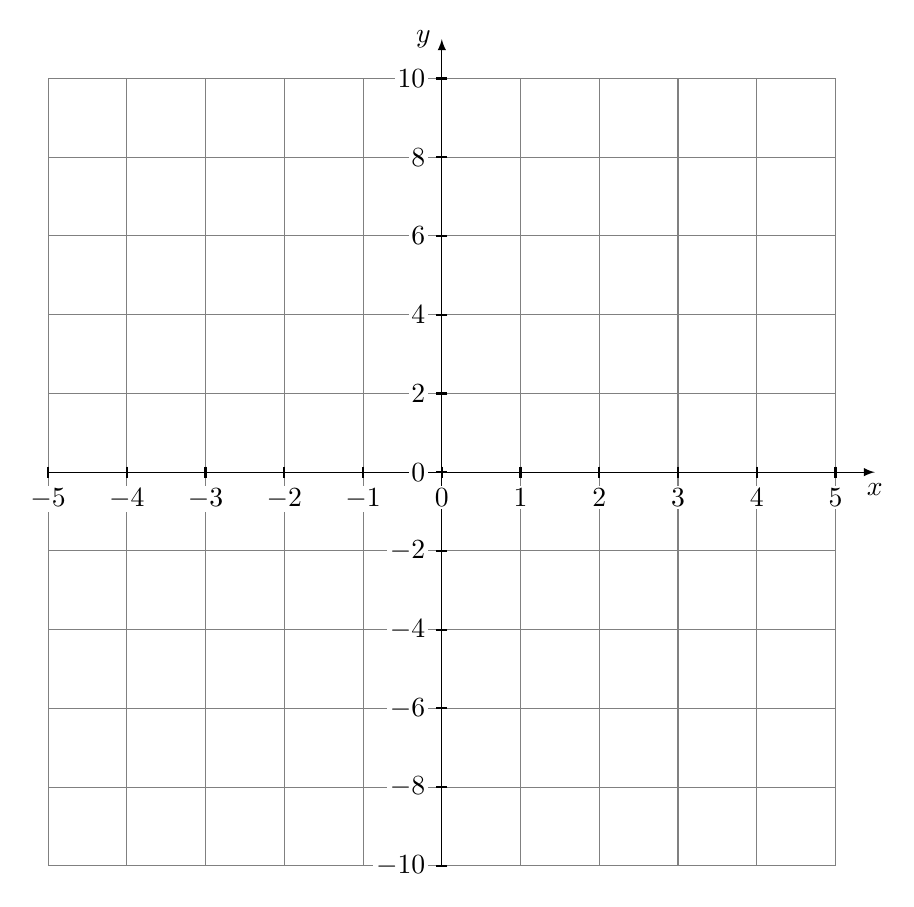
\begin{tikzpicture}[scale=1.0]
      \tkzInit[xmin=-5,xmax=5,ymin=-10,ymax=10,ystep=2]
      \tkzGrid
      \tkzAxeXY
      %\tkzFct[color=blue,thick,domain = -5:5]{x**3+2*x**2-5*x-6};
    \end{tikzpicture}

    \item What is the sign of the leading coefficient, positive or negative? Hence, what is the function's end behavior?
    \begin{enumerate}
        \item As $x\xrightarrow{}+\infty$ does $y\xrightarrow{}+\infty \text{ or } -\infty$?
        \item As $x\xrightarrow{}-\infty$ does $y\xrightarrow{}\infty \text{ or } -\infty$?
    \end{enumerate}
    \item Using the intercepts and end behavior, sketch the curve.
    \item Graph the function on a calculator. Is the shape of your sketch approximately correct?
\end{enumerate}

\newpage
Simplify

\item $(x +5)(3x-2)$\\*[50pt]
\item $(x -1)(x+2)(x-3)$\\*[50pt]

\item $x^3 \times x^{-2}y^2$\\*[50pt]
\item $x^3 \div x^{5}y$\\*[50pt]

\item $\sqrt[3]{x^6y^3z^6}$\\*[50pt]

The formula for simple interest is $P(t)=P_0(1+rt)$.
\item   What is the value of \$200 in principal at a rate of 5\%  per annum after one-half year?\\*[60pt]
\item   What is the value of \$220 in principal at a rate of 5.5\%  per annum after nine months?

\end{enumerate}

\end{document}
